\documentclass[a4paper,11pt]{article}
\usepackage[utf8]{inputenc}
\usepackage[spanish]{babel}
\usepackage[affil-it]{authblk}
\usepackage{enumerate}
\usepackage{graphicx}
\usepackage{hyperref}
\usepackage{amsmath}
\usepackage{amssymb}
\usepackage{cancel}
\usepackage[usenames, dvipsnames]{color}
\usepackage{tikz}
\usepackage[labelfont=bf]{caption}
\usepackage{subcaption} %Multiple images
\usepackage{multicol} % Multiple columns
\usepackage{float}
\usepackage{cleveref}
\usepackage{relsize} % bigger math symbols
\usepackage[margin=1.1in]{geometry}
\usepackage[titletoc,toc,title]{appendix}
\usepackage{enumitem}
\usepackage{etoolbox}
\usepackage{mdframed} %frame theorems
\usetikzlibrary{calc}
\numberwithin{equation}{section}

% Big Pictures
\usepackage[export]{adjustbox}

% Enviroment for theorems
\newmdtheoremenv[frametitle=Teorema]{theo}{Theorem}

% Circled words
\newcommand{\circled}[2][]{%
  \tikz[baseline=(char.base)]{%
    \node[shape = circle, draw, inner sep = 1pt]
    (char) {\phantom{\ifblank{#1}{#2}{#1}}};%
    \node at (char.center) {\makebox[0pt][c]{#2}};}}
\robustify{\circled}

%Appendices in spanish
\renewcommand{\appendixname}{Ap\'endices}
\renewcommand{\appendixtocname}{Ap\'endices}
\renewcommand{\appendixpagename}{Ap\'endices}

%Zero delimiter
\newcommand{\zerodel}{.\kern-\nulldelimiterspace}

%Columns separation
\setlength{\columnsep}{1cm}

%Indentation
\setlength{\parindent}{0ex}

%Multiple References

\crefrangelabelformat{equation}{(#3#1#4--#5\crefstripprefix{#1}{#2}#6)}

\usepackage{xparse}

%Boxes

\newcommand*{\boxcolor}{blue}
\makeatletter
\renewcommand{\boxed}[1]{\textcolor{\boxcolor}{%
\tikz[baseline={([yshift=-1ex]current bounding box.center)}] \node [rectangle, minimum width=1ex,rounded corners,draw] {\normalcolor\m@th$\displaystyle#1$};}}
 \makeatother

%Constantes
\newcommand{\euler}{\mathrm{e}}
\newcommand{\im}{i}

%Lemas, teoremas, definiciones y pruebas
\newcommand{\definicion}{\textbf{Definición: }}
\newcommand{\lema}{\textbf{Lema: }}
\newcommand{\teorema}{\textbf{Teorema: }}
\newcommand{\prueba}{\textbf{Prueba: }}
\newcommand{\proposicion}{\textbf{Proposición: }}
\newcommand{\corolario}{\textbf{Corolario: }}

% Definición de las secciones y su numeración

\makeatletter
\def\@seccntformat#1{%
  \expandafter\ifx\csname c@#1\endcsname\c@section\else
  \csname the#1\endcsname\quad
  \fi}
\makeatother

\begin{document}

\begin{titlepage}

\newcommand{\HRule}{\rule{\linewidth}{0.5mm}} % Defines a new command for the horizontal lines, change thickness here

\center % Center everything on the page
 
%----------------------------------------------------------------------------------------
%	HEADING SECTIONS
%----------------------------------------------------------------------------------------

\textsc{\LARGE Universidad Nacional Autónoma de México}\\[0.3cm] % Name of your university/college


\includegraphics[scale=0.17]{unam}

\textsc{\Large Electrodinámica Clásica}\\[0.5cm] % Major heading such as course name
\textsc{\large Semestre 2016-II}\\[0.5cm] % Minor heading such as course title

%----------------------------------------------------------------------------------------
%	TITLE SECTION
%----------------------------------------------------------------------------------------

\HRule \\[0.4cm]
{ \huge \bfseries Tarea \# 3. Campos Multipolares.}\\[0.2cm] % Title of your document
\HRule \\[1cm]
 
%----------------------------------------------------------------------------------------
%	AUTHOR SECTION
%----------------------------------------------------------------------------------------

\center
\large
\emph{Autor:} \\ % Your name
\Large Favio \textsc{Vázquez}\footnote{\href{mailto:favio.vazquez@correo.nucleares.unam.mx}{favio.vazquez@correo.nucleares.unam.mx}}


% If you don't want a supervisor, uncomment the two lines below and remove the section above
%\Large \emph{Author:}\\
%John \textsc{Smith}\\[3cm] % Your name

%----------------------------------------------------------------------------------------
%	COOL IMAGE SECTION
%----------------------------------------------------------------------------------------

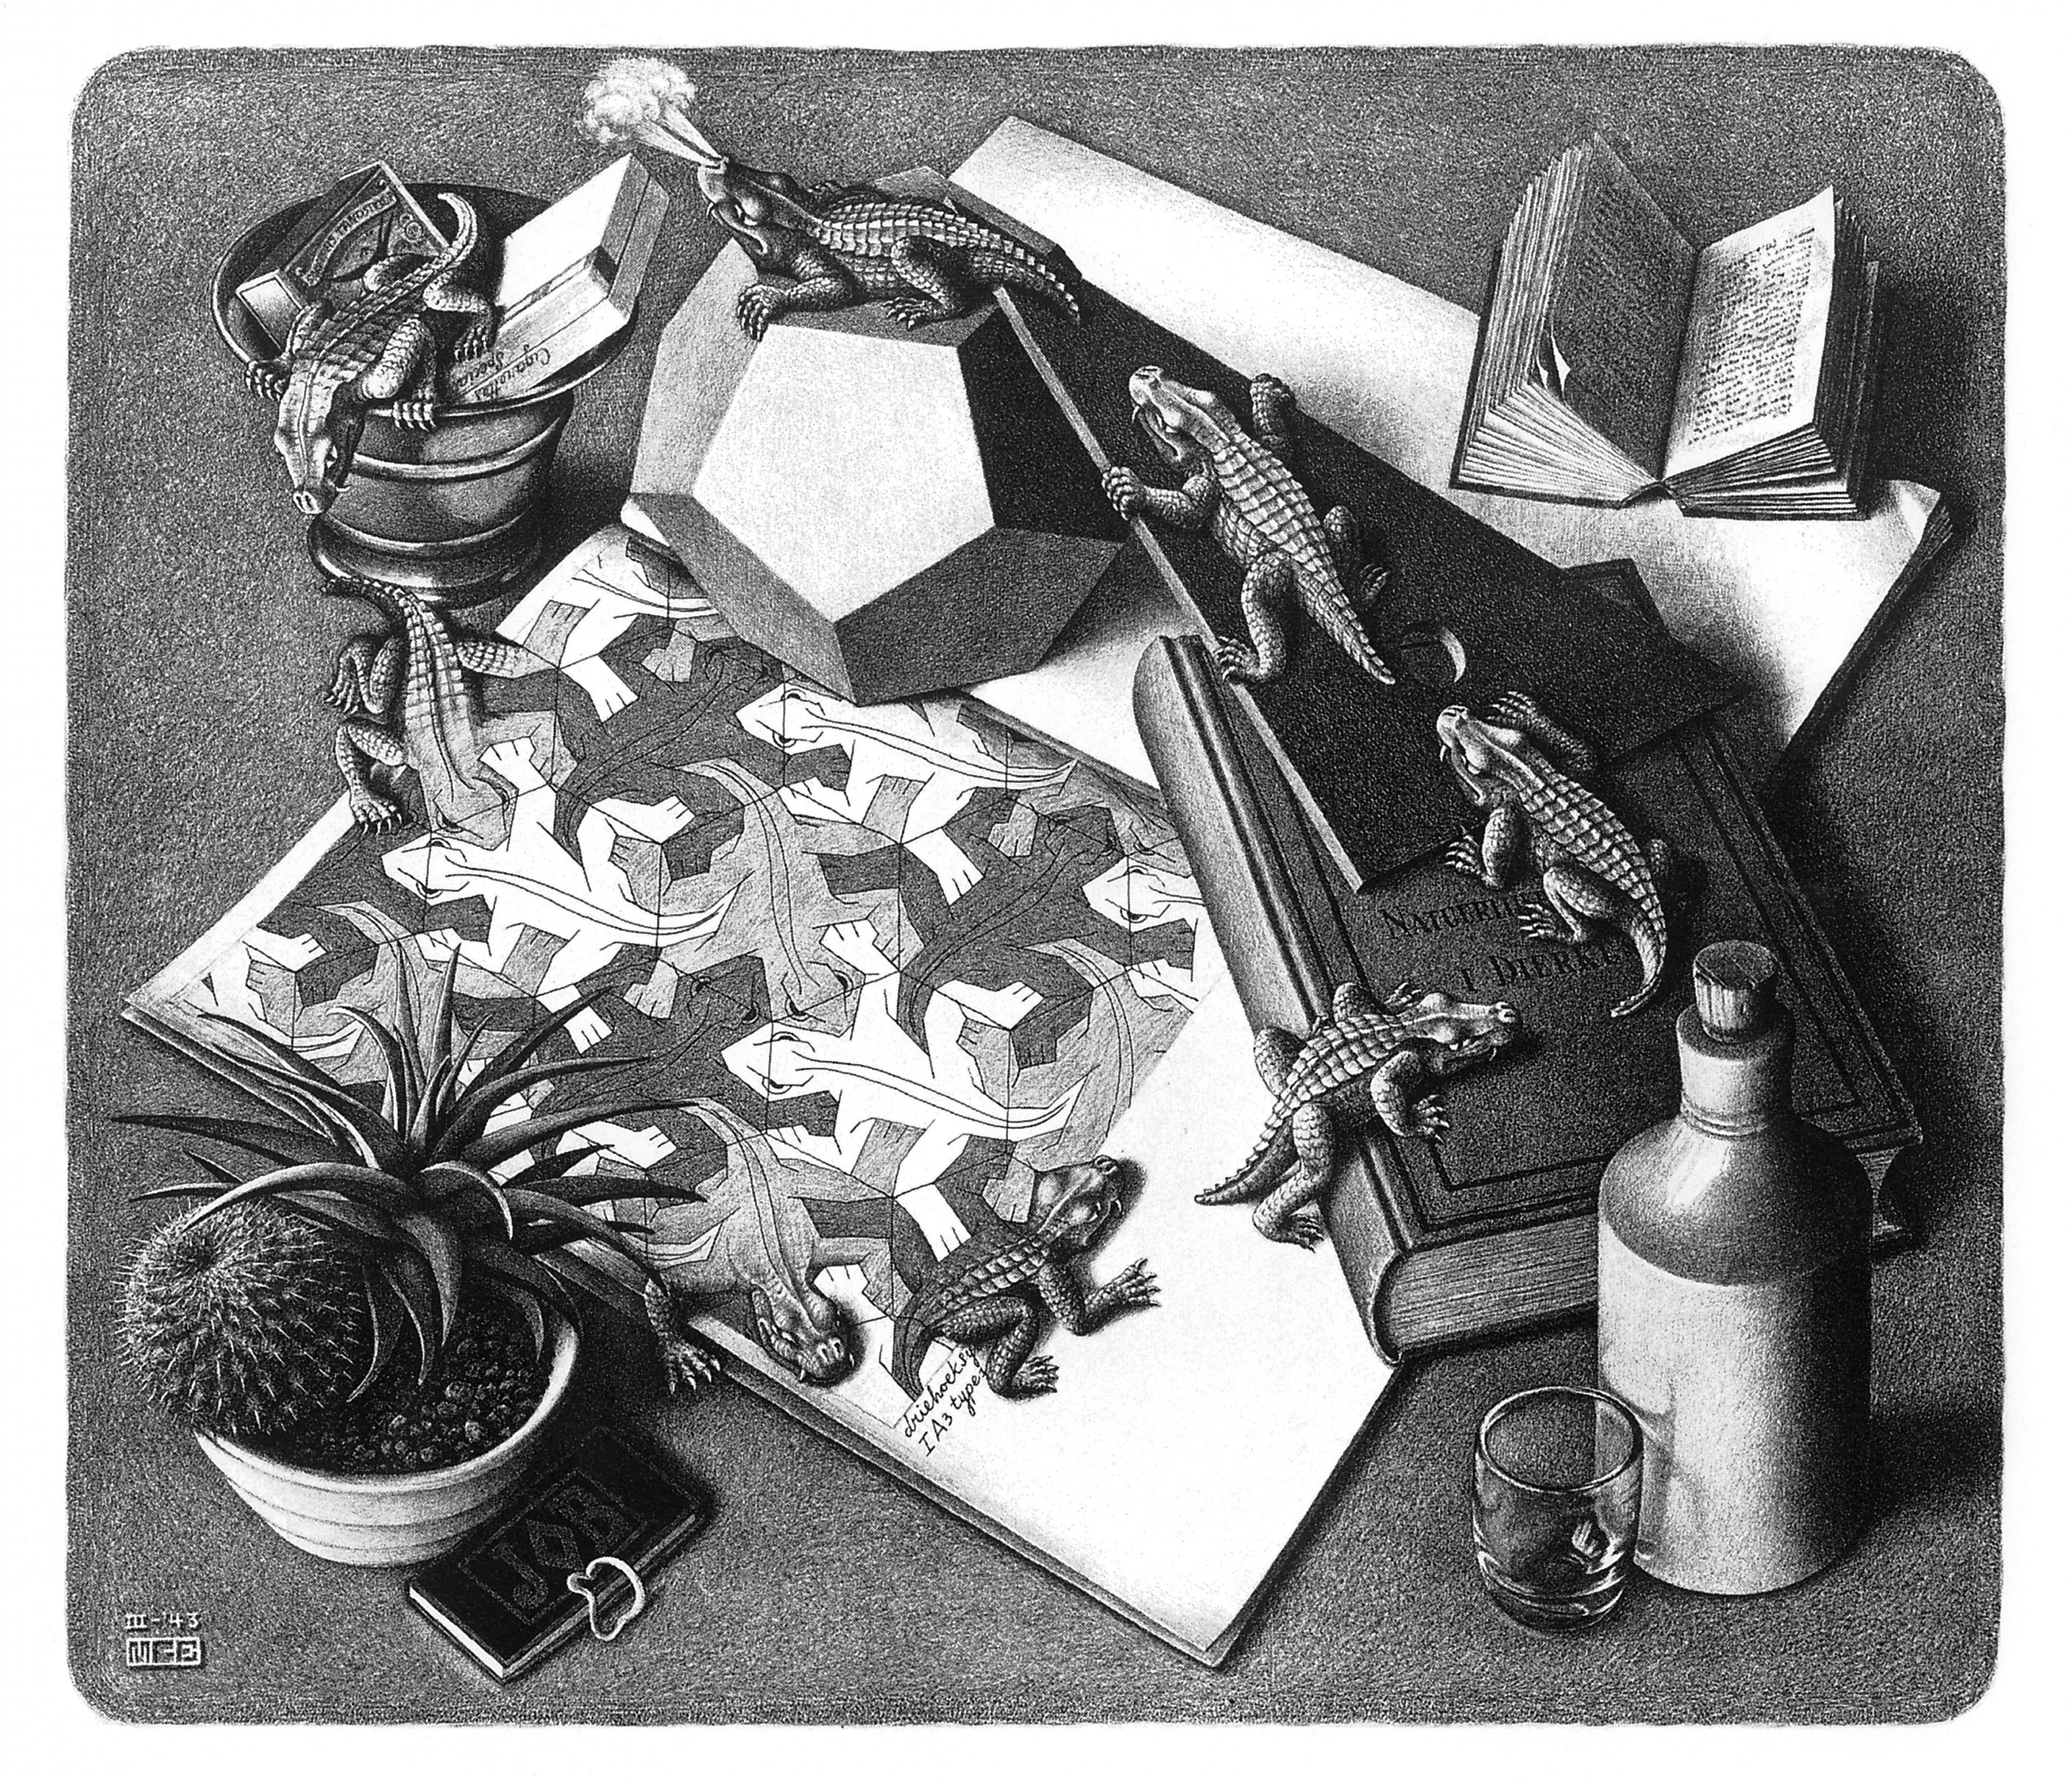
\includegraphics[scale=0.135]{reptilesEscher}

%----------------------------------------------------------------------------------------
%	LOGO SECTION
%----------------------------------------------------------------------------------------

%\includegraphics{logo.png}\\[1cm] % Include a department/university logo - this will require the graphicx package
 
%----------------------------------------------------------------------------------------

\vfill % Fill the rest of the page with whitespace

\end{titlepage}

\section{Problema 1. Problema 2.1 de Classical Electromagnetic Radiation
de Marion y Heald \cite{marion2}.}

Muestre que el campo eléctrico en el eje polar de un dipolo $\mathbf{p}$ es 
$2\mathbf{p}/z^3$, mientras que en el plano ecuatorial es $-\mathbf{p}/r^3$. Use 
este argumento elemental para mostrar, resolviendo el dipolo en dos componentes, que 
el campo en un punto arbitrario es 

$$
E(r,\theta) = \frac{p(2\cos{\theta}\mathbf{e_r} + \sen{\theta}\mathbf{e_\theta})}{r^3}
$$

\vspace{.3cm}

\underline{Solución:} \vspace{.3cm}

\section{Problema 2. Problema 2.2 de Classical Electromagnetic Radiation
de Marion y Heald \cite{marion2}.}

El campo magnético de la Tierra es aproximadamente el de un dipolo. Calcule el momento 
dipolar magnético usando el hecho de que la componente horizontal del campo de la 
Tierra en su superficie es aproximadamente $0.23$ G a una latitud magnética de 
$40^\circ$.

\vspace{.3cm}

\underline{Solución:} \vspace{.3cm}

\section{Problema 3. Problema 2.3 de Classical Electromagnetic Radiation
de Marion y Heald \cite{marion2}.}

Muestre que el momento dipolar eléctrico de un sistema de cargas es independiente 
de la elección del origen si el sistema tiene carga neta igual a cero.

\vspace{.3cm}

\underline{Solución:} \vspace{.3cm}

\section{Problema 4. Problema 2.3 de Classical Electromagnetic Radiation
de Marion y Heald \cite{marion2}.}

Muestre que la fuerza en un dipolo eléctrico es $\mathbf{F} = (\mathbf{p}\cdot 
\mathbf{grad})\mathbf{E}$. Luego considere la interacción de una carga $q$ y un dipolo 
$\mathbf{p}$ que están a una distancia $r$, con el dipolo orientado perpendicular a 
la línea que los une. Calcule la fuerza (vectorial)

\begin{enumerate}[label=\textbf{(\alph*)}]
\item en q debido a $\mathbf{p}$, 
\item en $\mathbf{p}$ debido a q.
\end{enumerate}

Si tus resultados violan la tercera ley de Newton, inténtalo de nuevo.

\vspace{.3cm}

\underline{Solución:} \vspace{.3cm}

\section{Problema 5. Problema 2.5 de Classical Electromagnetic Radiation
de Marion y Heald \cite{marion2}.}

Muestra que un dipolo finito simple (cargas $\pm q$ localizadas en $z = \pm l/2$) 
tiene un momento cuadrupolar cero con respecto a su centro como origen.

\vspace{.3cm}

\underline{Solución:} \vspace{.3cm}

\section{Problema 6. Problema 2.6 de Classical Electromagnetic Radiation
de Marion y Heald \cite{marion2}.}

Una carga $q_1 = + 2e$ está localizada en el origen y una carga $q_2 = - e$ está 
localizada en el punto $(x,y) = (1,0)$. Calcule el potencial en los puntos $(0,5)$
y $(5,0)$ en las siguientes maneras:

\begin{enumerate}[label=\textbf{(\alph*)}]
\item Mediante un cálculo directo de $q/R$ para cada carga,
\item Considerando un término de una expansión multipolar:
\subitem - De dos términos,
\subitem - De tres términos.
\end{enumerate}

Discute la diferencia en las tasas de convergencia hacia los valores exactos para 
los dos diferentes puntos del campo.

\vspace{.3cm}

\underline{Solución:} \vspace{.3cm}

\section{Problema 7. Problema 2.7 de Classical Electromagnetic Radiation
de Marion y Heald \cite{marion2}.}

Computa el tensor cuadrupolar para la siguiente distribución de cargas:

\begin{figure}[H]
\center
 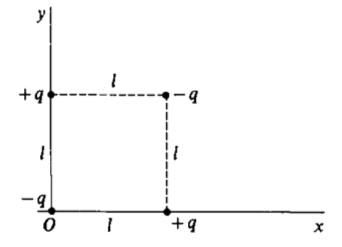
\includegraphics[scale=0.6]{problema7fig1}
\end{figure}

Diagonaliza el tensor mediante una rotación de coordenadas y encuentra el momento
cuadrupolar.

\vspace{.3cm}

\underline{Solución:} \vspace{.3cm}

\section{Problema 8. Problema 2.12 de Classical Electromagnetic Radiation
de Marion y Heald \cite{marion2}.}

La densidad de carga lineal de un anillo de radio $a$ está dada por 

$$
\lambda = \frac{q}{a}(\cos{\phi} - \sen{2\phi})
$$

\begin{enumerate}[label=\textbf{(\alph*)}]
\item Encontrar el momento monopolar, dipolar y cuadrupolar del sistema.
\item Calcular el potencial en un punto arbitrario del espacio, preciso hasta 
términos en $q/r^3$.
\end{enumerate}

\vspace{.3cm}

\underline{Solución:} \vspace{.3cm}

\begin{thebibliography}{10}
\bibitem{marion2}
J. Marion, M. Heald, \emph{Classical Electromagnetic Radiation}, 2da edición, Academic 
Press, 1965.
\end{thebibliography}

\end{document}